\chapter{前言：从滑模控制到非光滑系统}\label{ch:intro}

非线性动态系统理论是滑模控制的重要理论基础，也是我学习滑模的最大障碍。
我决定花一些时间从工科本科数学知识出发整理非光滑（非连续）动态系统中的一些概念。
这篇笔记首先回顾连续性与 Lipschitz 连续的定义，说明传统连续可微的 classical 解在应对非连续系统时存在性与唯一性上的缺陷，然后再引入 Filippov 等非光滑解概念。

\section{引子：一个绕不开的问题}

最近在看滑模控制的文章，其中对于非连续系统的论述多有不解，比如如下 Filippov 微分包含到底是什么，比如我总是可以看到 Filippov 这个定义，但是却对里面的数学分析、控制理论术语一窍不通。
\begin{quote}
  Filippov 微分包含的解的所有广为人知的性质(existence, extendability
  etc)但是不包含唯一性(uniqueness)。
\end{quote}
因此，我决定参考网络上的一些资料
\begin{enumerate}
  \item
    知乎讨论：请问filippov解大概是什么意思？是怎么定义的？有什么作用？
    \url{https://www.zhihu.com/question/55951952} 文中推荐参看\cite{cortesDiscontinuousDynamicalSystems2008,hanTheoryControlSystems2016}
  \item
    我检索到的一些文献，做一个简单的梳理。
    本文中关于解的存在唯一性的主要依据是 Khalil 的两本教材：
    \cite{khalilNonlinearSystems}（第三版，下称“Khalil 2002”）与
    \cite{khalilNonlinearControl2015}（下称“Khalil 2015”）。
\end{enumerate}
第\ref{ch:bounded}章关于非连续系统解的定义与存在性讨论，主要是翻译自 \cite{cortesDiscontinuousDynamicalSystems2008}。

\section{本书的阅读路线}\label{sec:reading-guide}

整本笔记围绕一个问题展开：\textbf{当控制器（或系统右端）不再连续时，微分方程的“解”到底是什么，稳定性又该如何定义？}
为此，笔记按“先连续、后非连续”的顺序组织，见表~\ref{tab:roadmap}。

\begin{table}[!htb]
  \centering
  \small
  \begin{tabular}{@{}c|p{5.6cm}|p{7.0cm}@{}}
    \hline
    章节 & 内容 & 回答的问题 \\
    \hline
    第\ref{ch:intro}章 & 前言、符号约定、连续性谱系 & 连续、一致连续、绝对连续、Lipschitz 连续之间是什么关系？\\
    \hline
    第\ref{ch:lipschitz}章 & 非线性系统：右端 Lipschitz 连续 & 经典解在什么条件下存在且唯一？为什么它只是“入场券”？\\
    \hline
    第\ref{ch:bounded}章 & 非光滑控制系统：右端有界 & 右端不连续时，用 Carathéodory / Filippov / sample-and-hold 如何定义解？稳定性怎么证？\\
    \hline
    第\ref{ch:case}章 & 一阶 bang-bang 案例 & Utkin 等效控制与 Filippov 微分包含各自成立的条件与边界在哪里？\\
    \hline
    第\ref{ch:sta}章 & 经典 STA 算法（草稿） & 具体算法层面的增益条件与 Lyapunov 证明 \\
    \hline
  \end{tabular}
  \caption{全书阅读路线}
  \label{tab:roadmap}
\end{table}

其中的逻辑主线是：

\begin{enumerate}
  \item 经典（classical）解要求右端函数关于状态\textbf{局部 Lipschitz 连续}，这就是第\ref{ch:lipschitz}章的主题；
  \item 滑模控制中的 $\sgn{s}$、bang-bang 控制、继电器等恰恰\textbf{破坏}了 Lipschitz 条件，于是经典解可能不存在、不唯一，必须换一套解的定义，这是第\ref{ch:bounded}章的主题；
  \item 新解的定义会带来新的“链式法则”问题（非光滑 Lyapunov 函数），于是需要 Dini 导数、Clarke 广义梯度与集值 Lie 导数；
  \item 最后用最简单的一阶系统把上述概念串起来，辨析 Utkin 等效控制与 Filippov 微分包含的适用边界（第\ref{ch:case}章）。
\end{enumerate}

建议第一次阅读时跳过标为“证明思路”的部分，先建立“右端越不光滑，需要的数学工具越重”这一直觉，再回头补证明。

\section{符号约定}\label{sec:notation}

本笔记尽量沿用 \cite{khalilNonlinearSystems} 的符号习惯，常用记号见表~\ref{tab:notation}。

\begin{table}[!htb]
  \centering
  \small
  \begin{tabular}{c|p{10cm}}
    \hline
    记号 & 含义 \\
    \hline
    $\RR$, $\RR^n$ & 实数集、$n$ 维实向量空间 \\
    $\norm{x}$ & 向量 $x$ 的 2-范数 $\sqrt{x^\top x}$；对矩阵为诱导范数 \\
    $B(x_0,r)$ 或 $N(x_0,r)$ & 以 $x_0$ 为心、$r$ 为半径的开球 $\{x:\norm{x-x_0}<r\}$ \\
    $\overline{co}(S)$ & 集合 $S$ 的凸闭包（convex closure） \\
    $C^k$, $C^\infty$ & $k$ 阶连续可微、光滑函数类 \\
    $D^+ V(t)$ & $V$ 的上右 Dini 导数（见第\ref{ch:bounded}章） \\
    $\partial V(x)$ & Clarke 广义梯度（见第\ref{ch:bounded}章） \\
    $\dot{\tilde V}$ & Shevitz--Paden 集值 Lie 导数（见第\ref{ch:bounded}章） \\
    $\mathbb{K}[f](x)$ & $f$ 在 $x$ 处的 Filippov 集值化 \\
    \hline
  \end{tabular}
  \caption{常用记号}
  \label{tab:notation}
\end{table}

全文默认 $x\in\RR^n$，$t\geq 0$，$f(t,x)$ 取值于 $\RR^n$；
$t$ 表示时间，$x$ 表示状态，$u$ 表示控制输入，$s$ 表示滑模变量。

\subsection{分数幂奇函数}

本文常用的符号为符号函数和 sig 函数，对于标量，其几何意义为符号函数，对于标量其定义为：
\begin{equation}
    \sig{x}^0=\sgn{x}=\begin{cases}
    	1   & x>0\\
    	-1 & x<0\\
    	0  & x=0\\
    \end{cases}
\end{equation}
基于此，我们定义 $\sig{x}^q=|x|^q \sgn{x}$。

类似的，相关定义可以拓展到向量形式，其几何意义为向量 $\vec{x}$ 的单位向量：
\begin{equation}
	\sig{\vec{x}}^0=\sgn{\vec{x}}=\begin{cases}
		\frac{\vec{x}}{\norm{\vec{x}}}, & \norm{\vec{x}}\neq 0\\
		\vec{0}   & \norm{\vec{x}}=0
	\end{cases}
\end{equation}
基于此，我们定义 $\sig{\vec{x}}^q=\|\vec{x}\|^q \sgn{\vec{x}}$。

下面介绍对几个常见的求导运算，使用多维向量的情况。
\begin{equation}
	\frac{\dd}{\dd t} \norm{\vec{x}}
	= \frac{\dd}{\dd t} \sqrt{\vec{x}^T\vec{x}}
	= \frac12 \frac{1}{\sqrt{\vec{x}^T\vec{x}}}\frac{\dd}{\dd t} {\vec{x}^T\vec{x}}
	= \frac12 \frac{1}{\sqrt{\vec{x}^T\vec{x}}} (2 \vec{x}^T \dot{\vec{x}})
	= \frac{\vec{x}^T\dot{\vec{x}}}{\norm{\vec{x}}}
\end{equation}
\begin{equation}
	\frac{\dd}{\dd t} \sig{\vec{x}}^q
	=\frac{\dd}{\dd t} \norm{\vec{x}}^{q-1} \vec{x}
	=\norm{\vec{x}}^{q-1} \dot{\vec{x}}+(q-1) \norm{\vec{x}}^{q-2}  \frac{\vec{x}^T\dot{\vec{x}}}{\norm{\vec{x}}}\vec{x}
\end{equation}
也就是说这里是基于向量的定义是难以求导的，这给一些从标量系统到向量的分析带来了困难。
\begin{equation}
	\frac{\dd}{\dd t} \sig{x}^q
	=|x|^{q-1} \dot{x}+(q-1) |x|^{q-2}  \frac{x \dot{x}}{|x|}x
	=q|x|^{q-1}\dot{x},
\end{equation}

\begin{remark}[$q=0$ 与 $q<1$ 的奇异性]
上面两式在 $q=0$ 与 $q<1$ 时在 $x=0$ 处不成立：
$q=0$ 时 $\sig{x}^0=\sgn{x}$ 在原点跳变；
$q=1/2$ 时导数 $q|x|^{q-1}$ 在原点无界（见图~\ref{fig:frac-power}）。
这正是超螺旋算法（STA）能在有限时间收敛、但也会带来抖振/数值刚性的根源：
它用“无限斜率”换取“有限时间”。
\end{remark}

\begin{figure}[!htb]
	\centering
	\begin{tikzpicture}
		\draw[->] (-2.2,0) -- (2.2,0) node[right] {$x$};
		\draw[->] (0,-1.8) -- (0,2.2) node[above] {$y$};
		\draw[domain=0:1.3,smooth,variable=\x,blue] plot ({\x},{\x*\x}); 
		\draw[domain=-1.3:0,smooth,variable=\x,blue] plot ({\x},{-\x*\x}); 
		\node[blue] at (2,2) {$y_1=\sig{x}^2$};
		\draw[domain=0:1.4,smooth,variable=\x,cyan] plot ({\x},{sqrt(\x)}); 
		\draw[domain=-1.4:0,smooth,variable=\x,cyan] plot ({\x},{-sqrt(-\x)}); 
		\node[cyan] at (2.4,1) {$y_2=\sig{x}^{1/2}$};
	\end{tikzpicture}
	\quad
	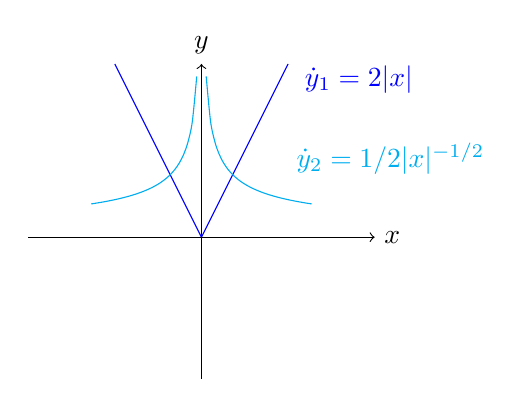
\begin{tikzpicture}
		\draw[->] (-2.2,0) -- (2.2,0) node[right] {$x$};
		\draw[->] (0,-1.8) -- (0,2.2) node[above] {$y$};
		\draw[domain=0:1.1,smooth,variable=\x,blue] plot ({\x},{2*\x}); 
		\draw[domain=-1.1:0,smooth,variable=\x,blue] plot ({\x},{-2*\x}); 
		\node[blue] at (2,2) {$\dot{y}_1=2|x|$};
		\draw[domain=0.06:1.4,smooth,variable=\x,cyan] plot ({\x},{1/2*1/sqrt(\x)}); 
		\draw[domain=-1.4:-0.06,smooth,variable=\x,cyan] plot ({\x},{1/2*1/sqrt(-\x)}); 
		\node[cyan] at (2.4,1) {$\dot{y}_2=1/2|x|^{-1/2}$};
	\end{tikzpicture}
	\caption{两个分数幂函数及其导数}
	\label{fig:frac-power}
\end{figure}

\subsection{常用不等式}\label{sec:inequalities}

后续证明反复用到下面几个不等式。

\begin{lemma}[Young 不等式]\label{lem:young}
对任意 $a,b\geq 0$ 与任意 $\varepsilon>0$，有
\begin{equation}
  2ab \leq \varepsilon a^2 + \frac{b^2}{\varepsilon},
  \qquad\text{等价地}\qquad
  ab \leq \frac{a^p}{p}+\frac{b^q}{q}\ \ (p,q>1,\ \tfrac1p+\tfrac1q=1).
\end{equation}
\end{lemma}

\begin{remark}[一个常用的变体]\label{rem:young-variant}
由 Lemma~\ref{lem:young}，对任意 $\mu>0$ 与 $z\in\RR$、$|s|>0$，取 $a=|z|$、$b=1$、$\varepsilon=\mu^{-1/2}$ 可得
\begin{equation}
  \frac{|z|^2}{\sqrt{|s|}} \geq -\mu^{-1}\sqrt{|s|} + 2\mu^{-1/2}|z| .
\end{equation}
两边同乘 $\sqrt{|s|}$ 即化为 $|z|^2 \ge -\mu^{-1}|s| + 2\mu^{-1/2}|z|\sqrt{|s|}$，
这正是 AM--GM 不等式。该式在 STA 的 Lyapunov 证明中用于处理交叉项。
\end{remark}

\begin{lemma}[Gronwall--Bellman 不等式]\label{lem:gronwall}
设 $u(t),v(t)$ 是 $[a,b]$ 上的非负连续函数，$c\geq 0$，且
\begin{equation}
  u(t) \le c + \int_a^t v(s)u(s)\,\dd s,\qquad t\in[a,b],
\end{equation}
则
\begin{equation}
  u(t) \le c\exp\left(\int_a^t v(s)\,\dd s\right),\qquad t\in[a,b].
\end{equation}
\end{lemma}

Gronwall 不等式是第\ref{ch:lipschitz}章证明唯一性与连续依赖性的核心工具，
也是滑模控制中估计“扰动下的偏差”的标准手段。




\section{回顾：连续性}\label{ux56deux987eux8fdeux7eedux6027}

那么什么是Lipschitz连续呢，各种连续的关系又是什么呢，我们讨论的非连续动态微分方程又如何定义呢？
为了简便，这里用的是函数来叙述，实际控制理论中大多为多维到多维的向量函数。如果是多变量函数或者泛函需要使用范数替代绝对值。

可微必可导。
可微是可导的充分条件。
只不过在一元情况下，由于两点确定一条直线，导致可微的线性替代就相当于求导（斜率确定 点确定 相当于直线确定）

\subsection{点连续与间断点}

\begin{definition}[点连续]
设函数\(y=f(x)\)在点\(x_0\)的某一邻域内有定义，
并且\(\lim_{x\to x_0}f(x)=f(x_0)\)，
那么就称函数\(f(x)\)在点\(x_0\)处连续。
\end{definition}

借此可以定义函数不连续和间断点的概念：
\begin{definition}
设函数\(f(x)\)在点\(x_0\)的某\textbf{去心}领域内有定义，
在此前提下，如果函数\(f(x)\)有一下三种情形之一 
\begin{enumerate}
  \item 在\(x=x_0\)处没有定义；
  \item 在\(x=x_0\)处有定义，但\(\lim_{x\to x_0} f(x)\)不存在；
  \item 在\(x=x_0\)处有定义，\(\lim_{x\to x_0} f(x)\)存在,但\(\lim_{x\to x_0}\neq f(x_0)\)
\end{enumerate}
那么函数\(f(x)\)在点\(x_0\)为不连续，\(x_0\)是函数\(f(x)\)的\textbf{间断点}。
\end{definition}



函数的间断点可以分为 
\begin{enumerate}
  \item 第一类间断点：左右极限都存在 
  \begin{enumerate}
    \item 可去间断点：左右极限都存在且相等 
    \item 跳跃间断点：左右极限都存在但不等 
  \end{enumerate}
  \item 第二类间断点：左右极限至少有一个不存在 
  \begin{enumerate}
    \item 震荡间断点：\(\lim_{x\to\ x_0} f(x)\)振荡不存在 
    \item 无穷间断点：\(\lim_{x\to\ x_0^+} f(x)=\infty\)或\(\lim_{x\to\ x_0^-} f(x)=\infty\)
  \end{enumerate}
\end{enumerate}


\begin{figure}[!hbp]
\centering
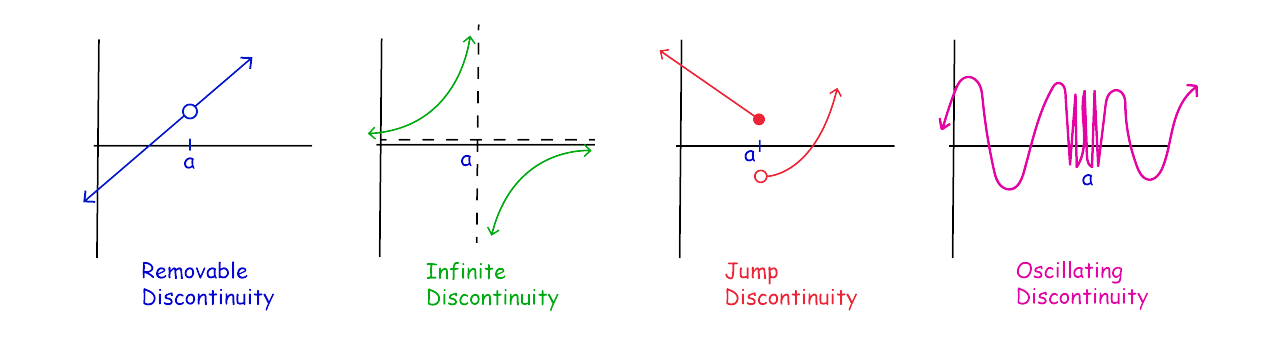
\includegraphics[width=\linewidth]{asserts/4-types-of-discontinuity.png}
\caption{
  间断点的定义与图示（来源：\url{https://calcworkshop.com/limits/limits-and-continuity/}）
}
\end{figure}

\subsection{连续性的关系}\label{subsec:continuity-relationships}

在闭区间\([a,b]\)上的实值函数中，连续性的包含关系为：
\[
\boxed{\text{光滑}(C^\infty)\subsetneq \text{连续可导}(C^1)\subsetneq \text{可导} \subsetneq \text{连续}}
\]
\[
\boxed{\text{Lipschitz连续} \subsetneq \text{绝对连续} \subsetneq \text{一致连续} = \text{连续}}
\]

在开区间上的实值函数中，连续性的包含关系为：
\[
\boxed{\text{光滑}(C^\infty)\subsetneq \text{连续可导}(C^1)\subsetneq \text{可导} \subsetneq \text{连续}}
\]
\[
\boxed{\text{Lipschitz连续} \subsetneq \text{绝对连续} \subsetneq \text{一致连续} \subsetneq \text{连续}}
\]

注意在开区间上两条链的每一环都是严格的（包括“一致连续\(\subsetneq\)连续”，因为Heine-Cantor定理此时不适用）。

\paragraph{两条链的联系与几乎处处可导}
\begin{itemize}
  \item 在闭区间上，连续可导（\(C^1\)）蕴含Lipschitz连续：导数连续故有界，从而\(|f(x_1)-f(x_2)|\le \sup|f'|\cdot|x_1-x_2|\)。但反之不成立（如\(f(x)=|x|\)是Lipschitz连续但在0处不可导）。即 \(C^1 \subsetneq \text{Lipschitz连续}\)。
  \item 对可导函数而言，导数处处有界 \(\iff\) Lipschitz连续。而 \(C^1 \subsetneq \{\text{可导且导数有界}\}\)，因为存在导数有界但导函数不连续的可导函数（如\(x^2\sin\frac{1}{x}\)在0附近）。
  \item \textbf{几乎处处可导}：Lipschitz连续函数几乎处处可导且导数几乎处处有界；绝对连续函数几乎处处可导且导数Lebesgue可积，并满足牛顿-莱布尼茨公式 \(f(t)=f(a)+\int_a^t f'(s)\,ds\)。注意“几乎处处可导”弱于“处处可导”，也不蕴含导数连续。
\end{itemize}

\begin{figure}[!htbp]
\centering
% =====================================================================
%  连续性关系图 —— 包含关系 / 蕴含关系总览
%
%  阅读约定
%   · 纵向自下而上：条件由弱到强（下方的集合更大）
%   · 箭头由强指向弱（$A\Rightarrow B$）；箭头旁的 $\subsetneq$ 按箭头方向
%     读作“箭尾集合 $\subsetneq$ 箭头集合”，灰色小字为其严格性的反例
%   · 蓝色 = 闭区间 $[a,b]$；红色 = 开区间 $(a,b)$；黑色 = 两种区间上关系相同
%   · 点线 = 非包含型蕴含（几乎处处可导、Rademacher / Lebesgue 定理）
%   · 有差别的边画蓝、红并列双箭头（两端接框）：红箭头上打 $\times$ = 开区间上不成立
%
%  用法: % =====================================================================
%  连续性关系图 —— 包含关系 / 蕴含关系总览
%
%  阅读约定
%   · 纵向自下而上：条件由弱到强（下方的集合更大）
%   · 箭头由强指向弱（$A\Rightarrow B$）；箭头旁的 $\subsetneq$ 按箭头方向
%     读作“箭尾集合 $\subsetneq$ 箭头集合”，灰色小字为其严格性的反例
%   · 蓝色 = 闭区间 $[a,b]$；红色 = 开区间 $(a,b)$；黑色 = 两种区间上关系相同
%   · 点线 = 非包含型蕴含（几乎处处可导、Rademacher / Lebesgue 定理）
%   · 有差别的边画蓝、红并列双箭头（两端接框）：红箭头上打 $\times$ = 开区间上不成立
%
%  用法: \input{asserts/continuity-relationship.tikz}
%  需要: \usepackage{tikz}\usetikzlibrary{arrows.meta}
% =====================================================================
\begin{tikzpicture}[
  % ---------- 节点 ----------
  cpt/.style={rectangle, rounded corners=2pt, draw=blue!45!black, thick, fill=white,
              align=center, minimum width=8.2em, minimum height=2.1em, inner sep=2.5pt,
              font=\footnotesize},
  % ---------- 箭头（箭头端 = 较弱 / 被蕴含者）----------
  %  蓝 = 闭区间 $[a,b]$；红 = 开区间 $(a,b)$；黑色 = 两种区间上关系相同
  arr/.style   ={-{Triangle[width=4.5pt,length=5.5pt]}, thick, blue!60!black},
  arrred/.style={-{Triangle[width=4.5pt,length=5.5pt]}, thick, red!80!black},
  aimp/.style  ={-{Triangle[width=4.5pt,length=5.5pt]}, thick, densely dotted, black!70},
  arrh/.style  ={{Triangle[width=4.5pt,length=5.5pt]}-{Triangle[width=4.5pt,length=5.5pt]},
                 thick, black!90},
  arrk/.style  ={-{Triangle[width=5.5pt,length=6.5pt]}, very thick, black!90},
  % ---------- 文字 ----------
  inel/.style={pos=0.5, right=3pt, anchor=west, font=\footnotesize, inner sep=1pt},
  inelr/.style={pos=0.5, left=3pt, anchor=east, font=\footnotesize, inner sep=1pt,
                text=red!80!black},
  cex/.style={font=\scriptsize, text=black!55, anchor=west, inner sep=1pt},
  cexr/.style={font=\scriptsize, text=red!80!black, anchor=east, align=right, inner sep=1pt},
  nbox/.style={draw=black!30, dashed, rounded corners=2pt, fill=black!2, align=left,
               font=\scriptsize, inner sep=3pt},
  xst/.style={font=\normalsize\bfseries, text=red!80!black, fill=white, inner sep=0.8pt},
]

% =====================================================================
%  主链（自上而下 = 由强到弱）：
%  解析 → C^\infty → C^1 → Lipschitz → Hölder → 绝对连续 → 一致连续 → 连续
% =====================================================================
\node[cpt] (c0) at (-2.2,  0.0) {连续 $C^0$};
\node[cpt] (c1) at (-2.2,  1.8) {一致连续};
\node[cpt] (c2) at (-2.2,  3.6) {绝对连续};
\node[cpt] (c3) at (-2.2,  5.4) {Hölder 连续};
\node[cpt] (c4) at (-2.2,  7.2) {Lipschitz 连续};
\node[cpt] (c5) at (-2.2,  9.0) {$C^1$ 连续可导};
\node[cpt] (c6) at (-2.2, 10.8) {光滑 $C^\infty$};
\node[cpt] (c7) at (-2.2, 12.6) {解析 $C^\omega$};

% =====================================================================
%  主链的边：
%   · 开、闭区间上关系相同的边：一条黑色粗箭头（通用）
%   · 两种区间上有差别的边：蓝、红两个并列箭头（$\pm0.45$cm，两端接框边），
%     蓝 = 闭区间 $[a,b]$，红 = 开区间 $(a,b)$，红箭头上 $\times$ = 开区间上不成立
% =====================================================================

% ---------- 一致连续 → 连续：闭区间 $=$（Heine–Cantor）；开区间 $\subsetneq$ ----------
\draw[arr] ([xshift=0.45cm]c1.south) -- ([xshift=0.45cm]c0.north) node[inel] {$=$};
\draw[arrred] ([xshift=-0.45cm]c1.south) -- ([xshift=-0.45cm]c0.north)
      node[inelr] {$\subsetneq$};
\node[cexr] at (-3.3, 0.9) {开区间更弱（Heine–Cantor 失效）\\如 $\sin\frac1x$ 在 $(0,1)$};

% ---------- 连续 → 有界：闭区间成立（有界性定理）；开区间不成立 ----------
\node[cpt] (bd) at (-2.2, -2.4) {有界};
\draw[arr] ([xshift=0.45cm]c0.south) -- ([xshift=0.45cm]bd.north)
      node[pos=0.5, right=4pt, cex] {有界性定理};
\draw[arrred] ([xshift=-0.45cm]c0.south) -- ([xshift=-0.45cm]bd.north)
      node[pos=0.5, xst] {$\times$};
\node[cexr] at (-3.3, -1.2) {开区间 $\not\Rightarrow$ 有界\\（$1/x$ 在 $(0,1)$ 无界）};

% ---------- 绝对连续 → 一致连续（两种区间上相同：黑粗箭头）----------
\draw[arrk] (c2) -- (c1)
      node[inel] {$\subsetneq$} node[pos=0.5, right=13pt, cex] {$x\sin\frac1x$};

% ---------- Hölder → 绝对连续（两种区间上相同：黑粗箭头）----------
\draw[arrk] (c3) -- (c2) node[inel] {$\subsetneq$};

% ---------- Lipschitz → Hölder（两种区间上相同：黑粗箭头）----------
\draw[arrk] (c4) -- (c3)
      node[inel] {$\subsetneq$} node[pos=0.5, right=13pt, cex] {$\sqrt{|t|}$};

% ---------- $C^1$ → Lipschitz：闭区间 $\subsetneq$；开区间不成立 ----------
\draw[arr] ([xshift=0.45cm]c5.south) -- ([xshift=0.45cm]c4.north)
      node[inel] {$\subsetneq$} node[pos=0.5, right=13pt, cex] {$|t|$};
\draw[arrred] ([xshift=-0.45cm]c5.south) -- ([xshift=-0.45cm]c4.north)
      node[pos=0.5, xst] {$\times$};
\node[cexr] at (-3.3, 8.1) {开区间 $\not\Rightarrow$ Lipschitz（$1/x$）};

% ---------- 光滑 → $C^1$（两种区间上相同：黑粗箭头）----------
\draw[arrk] (c6) -- (c5)
      node[inel] {$\subsetneq$}
      node[pos=0.5, right=13pt, cex] {$x^3\sin\frac1{x^2}$；$C^k$ 同理};

% ---------- 解析 → 光滑（两种区间上相同：黑粗箭头）----------
\draw[arrk] (c7) -- (c6)
      node[inel] {$\subsetneq$} node[pos=0.5, right=13pt, cex] {$e^{-1/x^2}$};

% =====================================================================
%  右支：处处可导 / 几乎处处可导
% =====================================================================
\node[cpt] (d0) at (2.0, 1.8) {处处可导};
\node[cpt] (ae) at (2.0, 5.4) {几乎处处可导};
\node[cpt] (aeb) at (2.0, 7.2) {a.e.\ 可导\\ 且 $|f'|\le L$ a.e.\\
      {\scriptsize （Rademacher 定理）}};

% ---------- C^1 的定义：可导 且 f' 连续 ----------
\node[cpt] (dc) at (2.0, 9.0) {可导且 $f'$ 连续};
\draw[arrh] (c5) -- (dc)
      node[midway, above=2pt, font=\footnotesize] {$=$\,定义};

% ---------- 可导 ⇒ 连续（与区间开、闭无关）：黑粗箭头 ----------
\draw[arrk] (d0) -- (c0) node[pos=0.55, above=1pt, font=\footnotesize, fill=white,
      inner sep=1pt] {$\subsetneq$};

\draw[aimp] (d0) -- (ae)
      node[pos=0.32, left=4pt, anchor=east, cex, fill=white] {a.e. 成立};
\draw[aimp] (c2) -- (ae) node[pos=0.68, above=1pt, font=\scriptsize, fill=white,
      inner sep=1pt] {Lebesgue 定理};
% ---------- Lipschitz ⇒ a.e. 可导 且导数 a.e. 有界 |f'| ≤ L ----------
\draw[aimp] (c4) -- (aeb);
\draw[arrk] (aeb) -- (ae)
      node[pos=0.5, right=3pt, font=\footnotesize, fill=white, inner sep=1pt] {$\subsetneq$};

% =====================================================================
%  注释 1（左）：绝对连续 = Lebesgue 原函数
% =====================================================================
\node[nbox] at (-5.95, 3.4) {%
  \textbf{绝对连续 $\iff$ Lebesgue 原函数}\\
  $f(t)=f(a)+\int_a^t f'(s)\,\mathrm{d}s$\\
  $f'\in L^1$（Newton–Leibniz）};

% =====================================================================
%  注释 2（左）：Hölder 的指数 α
% =====================================================================
\node[nbox] at (-5.95, 6.35) {%
  \textbf{Hölder $C^{0,\alpha}$}\\
  $|f(x)-f(y)|\le C|x-y|^{\alpha}$\\
  $\alpha=1$：即 Lipschitz\\
  $\alpha\to0^+$：只保证有界\\
  $\bigcup_{\alpha>0}C^{0,\alpha}\subsetneq$ 绝对连续};

% =====================================================================
%  注释 3（右上）：导数有界 ↔ Lipschitz，C^1 ⊊ {f' 有界}
% =====================================================================
\node[nbox] at (5.7, 10.0) {%
  \textbf{导数有界}\quad $f$ 处处可导时\\
  $f'\in L^\infty\iff$ Lipschitz\\
  $C^1\subsetneq\{f'\,\text{有界}\}$（$x^2\sin\frac1x$）\\
  开区间：$C^1\not\subset$ Lipschitz（$1/x$）};

% =====================================================================
%  注释 4（右下）：单调 / 有界变差 / a.e. 导数可积
% =====================================================================
\node[nbox] at (5.3, 3.9) {%
  \textbf{单调 $\Rightarrow$ BV $\Rightarrow$ a.e. 可导}\\
  BV：$f=g-h$（两单调函数之差）\\
  绝对连续 $\subsetneq$ BV，BV $\Rightarrow f'\in L^1$\\
  a.e. 可导 $\not\Rightarrow f'\in L^1$};

% =====================================================================
%  注释 5（右下）：与微分方程解的联系（经典解 / Filippov 解）
% =====================================================================
\node[nbox] at (4.6, -1.7) {%
  \textbf{与 $\dot x=f(x)$ 解的联系}\\
  经典解 $x(t)\in C^1$：要求 $f$ 连续\\
  Filippov 解 $x(t)$ 绝对连续：\\
  \quad $f$ 可测、局部本质有界\\
  唯一性：$f$ 局部 Lipschitz};

% =====================================================================
%  图例（左上空白区）
% =====================================================================
\node[font=\scriptsize\bfseries, anchor=west] at (-7.8, 12.9) {图例（箭头由强到弱）};
\draw[arrk]   (-7.8, 12.3) -- (-7.0, 12.3);
\node[cex, text=black] at (-6.85, 12.3) {黑：两种区间上相同};
\draw[arr]    (-7.8, 11.7) -- (-7.0, 11.7);
\node[cex, text=black] at (-6.85, 11.7) {蓝色：闭区间 $[a,b]$};
\draw[arrred] (-7.8, 11.1) -- (-7.0, 11.1);
\node[cex, text=black] at (-6.85, 11.1) {红色：开区间 $(a,b)$};
\draw[aimp]   (-7.8, 10.5) -- (-7.0, 10.5);
\node[cex, text=black] at (-6.85, 10.5) {点线：非包含型蕴含};
\draw[arrh]   (-7.8,  9.9) -- (-7.0,  9.9);
\node[cex, text=black] at (-6.85,  9.9) {$=$：定义 / 等价};
\node[cex, text=black] at (-7.8,   9.3) {灰色小字：反例};
\draw[arrred] (-7.8, 8.7) -- (-7.0, 8.7);
\node[xst, font=\scriptsize\bfseries] at (-7.4, 8.7) {$\times$};
\node[cex, text=black] at (-6.85, 8.7) {开区间上不成立};

\end{tikzpicture}

%  需要: \usepackage{tikz}\usetikzlibrary{arrows.meta}
% =====================================================================
\begin{tikzpicture}[
  % ---------- 节点 ----------
  cpt/.style={rectangle, rounded corners=2pt, draw=blue!45!black, thick, fill=white,
              align=center, minimum width=8.2em, minimum height=2.1em, inner sep=2.5pt,
              font=\footnotesize},
  % ---------- 箭头（箭头端 = 较弱 / 被蕴含者）----------
  %  蓝 = 闭区间 $[a,b]$；红 = 开区间 $(a,b)$；黑色 = 两种区间上关系相同
  arr/.style   ={-{Triangle[width=4.5pt,length=5.5pt]}, thick, blue!60!black},
  arrred/.style={-{Triangle[width=4.5pt,length=5.5pt]}, thick, red!80!black},
  aimp/.style  ={-{Triangle[width=4.5pt,length=5.5pt]}, thick, densely dotted, black!70},
  arrh/.style  ={{Triangle[width=4.5pt,length=5.5pt]}-{Triangle[width=4.5pt,length=5.5pt]},
                 thick, black!90},
  arrk/.style  ={-{Triangle[width=5.5pt,length=6.5pt]}, very thick, black!90},
  % ---------- 文字 ----------
  inel/.style={pos=0.5, right=3pt, anchor=west, font=\footnotesize, inner sep=1pt},
  inelr/.style={pos=0.5, left=3pt, anchor=east, font=\footnotesize, inner sep=1pt,
                text=red!80!black},
  cex/.style={font=\scriptsize, text=black!55, anchor=west, inner sep=1pt},
  cexr/.style={font=\scriptsize, text=red!80!black, anchor=east, align=right, inner sep=1pt},
  nbox/.style={draw=black!30, dashed, rounded corners=2pt, fill=black!2, align=left,
               font=\scriptsize, inner sep=3pt},
  xst/.style={font=\normalsize\bfseries, text=red!80!black, fill=white, inner sep=0.8pt},
]

% =====================================================================
%  主链（自上而下 = 由强到弱）：
%  解析 → C^\infty → C^1 → Lipschitz → Hölder → 绝对连续 → 一致连续 → 连续
% =====================================================================
\node[cpt] (c0) at (-2.2,  0.0) {连续 $C^0$};
\node[cpt] (c1) at (-2.2,  1.8) {一致连续};
\node[cpt] (c2) at (-2.2,  3.6) {绝对连续};
\node[cpt] (c3) at (-2.2,  5.4) {Hölder 连续};
\node[cpt] (c4) at (-2.2,  7.2) {Lipschitz 连续};
\node[cpt] (c5) at (-2.2,  9.0) {$C^1$ 连续可导};
\node[cpt] (c6) at (-2.2, 10.8) {光滑 $C^\infty$};
\node[cpt] (c7) at (-2.2, 12.6) {解析 $C^\omega$};

% =====================================================================
%  主链的边：
%   · 开、闭区间上关系相同的边：一条黑色粗箭头（通用）
%   · 两种区间上有差别的边：蓝、红两个并列箭头（$\pm0.45$cm，两端接框边），
%     蓝 = 闭区间 $[a,b]$，红 = 开区间 $(a,b)$，红箭头上 $\times$ = 开区间上不成立
% =====================================================================

% ---------- 一致连续 → 连续：闭区间 $=$（Heine–Cantor）；开区间 $\subsetneq$ ----------
\draw[arr] ([xshift=0.45cm]c1.south) -- ([xshift=0.45cm]c0.north) node[inel] {$=$};
\draw[arrred] ([xshift=-0.45cm]c1.south) -- ([xshift=-0.45cm]c0.north)
      node[inelr] {$\subsetneq$};
\node[cexr] at (-3.3, 0.9) {开区间更弱（Heine–Cantor 失效）\\如 $\sin\frac1x$ 在 $(0,1)$};

% ---------- 连续 → 有界：闭区间成立（有界性定理）；开区间不成立 ----------
\node[cpt] (bd) at (-2.2, -2.4) {有界};
\draw[arr] ([xshift=0.45cm]c0.south) -- ([xshift=0.45cm]bd.north)
      node[pos=0.5, right=4pt, cex] {有界性定理};
\draw[arrred] ([xshift=-0.45cm]c0.south) -- ([xshift=-0.45cm]bd.north)
      node[pos=0.5, xst] {$\times$};
\node[cexr] at (-3.3, -1.2) {开区间 $\not\Rightarrow$ 有界\\（$1/x$ 在 $(0,1)$ 无界）};

% ---------- 绝对连续 → 一致连续（两种区间上相同：黑粗箭头）----------
\draw[arrk] (c2) -- (c1)
      node[inel] {$\subsetneq$} node[pos=0.5, right=13pt, cex] {$x\sin\frac1x$};

% ---------- Hölder → 绝对连续（两种区间上相同：黑粗箭头）----------
\draw[arrk] (c3) -- (c2) node[inel] {$\subsetneq$};

% ---------- Lipschitz → Hölder（两种区间上相同：黑粗箭头）----------
\draw[arrk] (c4) -- (c3)
      node[inel] {$\subsetneq$} node[pos=0.5, right=13pt, cex] {$\sqrt{|t|}$};

% ---------- $C^1$ → Lipschitz：闭区间 $\subsetneq$；开区间不成立 ----------
\draw[arr] ([xshift=0.45cm]c5.south) -- ([xshift=0.45cm]c4.north)
      node[inel] {$\subsetneq$} node[pos=0.5, right=13pt, cex] {$|t|$};
\draw[arrred] ([xshift=-0.45cm]c5.south) -- ([xshift=-0.45cm]c4.north)
      node[pos=0.5, xst] {$\times$};
\node[cexr] at (-3.3, 8.1) {开区间 $\not\Rightarrow$ Lipschitz（$1/x$）};

% ---------- 光滑 → $C^1$（两种区间上相同：黑粗箭头）----------
\draw[arrk] (c6) -- (c5)
      node[inel] {$\subsetneq$}
      node[pos=0.5, right=13pt, cex] {$x^3\sin\frac1{x^2}$；$C^k$ 同理};

% ---------- 解析 → 光滑（两种区间上相同：黑粗箭头）----------
\draw[arrk] (c7) -- (c6)
      node[inel] {$\subsetneq$} node[pos=0.5, right=13pt, cex] {$e^{-1/x^2}$};

% =====================================================================
%  右支：处处可导 / 几乎处处可导
% =====================================================================
\node[cpt] (d0) at (2.0, 1.8) {处处可导};
\node[cpt] (ae) at (2.0, 5.4) {几乎处处可导};
\node[cpt] (aeb) at (2.0, 7.2) {a.e.\ 可导\\ 且 $|f'|\le L$ a.e.\\
      {\scriptsize （Rademacher 定理）}};

% ---------- C^1 的定义：可导 且 f' 连续 ----------
\node[cpt] (dc) at (2.0, 9.0) {可导且 $f'$ 连续};
\draw[arrh] (c5) -- (dc)
      node[midway, above=2pt, font=\footnotesize] {$=$\,定义};

% ---------- 可导 ⇒ 连续（与区间开、闭无关）：黑粗箭头 ----------
\draw[arrk] (d0) -- (c0) node[pos=0.55, above=1pt, font=\footnotesize, fill=white,
      inner sep=1pt] {$\subsetneq$};

\draw[aimp] (d0) -- (ae)
      node[pos=0.32, left=4pt, anchor=east, cex, fill=white] {a.e. 成立};
\draw[aimp] (c2) -- (ae) node[pos=0.68, above=1pt, font=\scriptsize, fill=white,
      inner sep=1pt] {Lebesgue 定理};
% ---------- Lipschitz ⇒ a.e. 可导 且导数 a.e. 有界 |f'| ≤ L ----------
\draw[aimp] (c4) -- (aeb);
\draw[arrk] (aeb) -- (ae)
      node[pos=0.5, right=3pt, font=\footnotesize, fill=white, inner sep=1pt] {$\subsetneq$};

% =====================================================================
%  注释 1（左）：绝对连续 = Lebesgue 原函数
% =====================================================================
\node[nbox] at (-5.95, 3.4) {%
  \textbf{绝对连续 $\iff$ Lebesgue 原函数}\\
  $f(t)=f(a)+\int_a^t f'(s)\,\mathrm{d}s$\\
  $f'\in L^1$（Newton–Leibniz）};

% =====================================================================
%  注释 2（左）：Hölder 的指数 α
% =====================================================================
\node[nbox] at (-5.95, 6.35) {%
  \textbf{Hölder $C^{0,\alpha}$}\\
  $|f(x)-f(y)|\le C|x-y|^{\alpha}$\\
  $\alpha=1$：即 Lipschitz\\
  $\alpha\to0^+$：只保证有界\\
  $\bigcup_{\alpha>0}C^{0,\alpha}\subsetneq$ 绝对连续};

% =====================================================================
%  注释 3（右上）：导数有界 ↔ Lipschitz，C^1 ⊊ {f' 有界}
% =====================================================================
\node[nbox] at (5.7, 10.0) {%
  \textbf{导数有界}\quad $f$ 处处可导时\\
  $f'\in L^\infty\iff$ Lipschitz\\
  $C^1\subsetneq\{f'\,\text{有界}\}$（$x^2\sin\frac1x$）\\
  开区间：$C^1\not\subset$ Lipschitz（$1/x$）};

% =====================================================================
%  注释 4（右下）：单调 / 有界变差 / a.e. 导数可积
% =====================================================================
\node[nbox] at (5.3, 3.9) {%
  \textbf{单调 $\Rightarrow$ BV $\Rightarrow$ a.e. 可导}\\
  BV：$f=g-h$（两单调函数之差）\\
  绝对连续 $\subsetneq$ BV，BV $\Rightarrow f'\in L^1$\\
  a.e. 可导 $\not\Rightarrow f'\in L^1$};

% =====================================================================
%  注释 5（右下）：与微分方程解的联系（经典解 / Filippov 解）
% =====================================================================
\node[nbox] at (4.6, -1.7) {%
  \textbf{与 $\dot x=f(x)$ 解的联系}\\
  经典解 $x(t)\in C^1$：要求 $f$ 连续\\
  Filippov 解 $x(t)$ 绝对连续：\\
  \quad $f$ 可测、局部本质有界\\
  唯一性：$f$ 局部 Lipschitz};

% =====================================================================
%  图例（左上空白区）
% =====================================================================
\node[font=\scriptsize\bfseries, anchor=west] at (-7.8, 12.9) {图例（箭头由强到弱）};
\draw[arrk]   (-7.8, 12.3) -- (-7.0, 12.3);
\node[cex, text=black] at (-6.85, 12.3) {黑：两种区间上相同};
\draw[arr]    (-7.8, 11.7) -- (-7.0, 11.7);
\node[cex, text=black] at (-6.85, 11.7) {蓝色：闭区间 $[a,b]$};
\draw[arrred] (-7.8, 11.1) -- (-7.0, 11.1);
\node[cex, text=black] at (-6.85, 11.1) {红色：开区间 $(a,b)$};
\draw[aimp]   (-7.8, 10.5) -- (-7.0, 10.5);
\node[cex, text=black] at (-6.85, 10.5) {点线：非包含型蕴含};
\draw[arrh]   (-7.8,  9.9) -- (-7.0,  9.9);
\node[cex, text=black] at (-6.85,  9.9) {$=$：定义 / 等价};
\node[cex, text=black] at (-7.8,   9.3) {灰色小字：反例};
\draw[arrred] (-7.8, 8.7) -- (-7.0, 8.7);
\node[xst, font=\scriptsize\bfseries] at (-7.4, 8.7) {$\times$};
\node[cex, text=black] at (-6.85, 8.7) {开区间上不成立};

\end{tikzpicture}

\caption{连续性诸概念之间的关系（蓝色：闭区间 $[a,b]$；红色：开区间 $(a,b)$ 上的差别；
  箭头由强到弱，即 $A\to B$ 表示 $A\Rightarrow B$，边上的 $\subsetneq$ 读作“箭尾集合 $\subsetneq$ 箭头集合”，
  $=$ 表示定义或等价；灰色小字为说明严格性的反例）}
\label{fig:continuity-poset}
\end{figure}


\subsection{区间连续与区间一致连续（连续、绝对连续、Lipschitz连续、Hölder连续）}

如果在区间上每一点都连续，就称函数在该区间上连续，如果区间包括端点，那么在右端点连续是指左连续，在左端点连续是指右连续。

\begin{definition}[一致连续]
设函数\(f(x)\)在区间\(I\)上有定义.
如果对于任意给定的正数\(\epsilon\)，总存在正数
\(\delta\)，使得对于区间\(I\)上的任意两点\(x_1,x_2\)，当\(|x_1-x_2|<\delta\)时，
有 \[
|f(x_1)-f(x_2)|<\epsilon
\] 那么称函数\(f(x)\)在区间\(I\)上\textbf{一致连续}。
\end{definition}

绝对连续表示函数的光滑性质，比连续和一致连续条件都要严格，比Lipschitz条件宽松，是一类极为重要的函数。绝对连续函数几乎处处可微，是它的导函数的广义原函数。

\begin{definition}[绝对连续]
设\(f(x)\)是\([a,b]\)上的函数，若对任意\(\epsilon>0\)，存在\(\delta>0\)使得对于
\([a,b]\)中的任意一组分点： \[
a_1<b_1\leq a_2 <b_2 \leq \dots \leq a_n < b_n,
\] 只要\(\sum_{i=1}^n(b_i-a_i)<\delta\)，便有 \[
\sum_{i=1}^n|f(b_i)-f(a_i)|<\epsilon
\]
则称\(f(x)\)是\([a,b]\)上\textbf{绝对连续}函数，或称\(f(x)\)在\([a,b]\)上绝对连续。
\end{definition}

等价的，如果存在一个Lebesgue可积函数\(k:[a,b]\to \mathbb{R}\)
使得下式成立，那么\(f\)是一个绝对连续函数。 \[
f(t)=f(a)+\int^t_a k(s)d s,\quad t\in [a,b]
\]

\begin{definition}[Lipschitz连续]
对于函数\(f(x)\)，如果存在一个常数L，使得对\(f(x)\)定义域上（可为实数也可以为复数）的任意两个值满足如下条件：
\[
|f(x_1)-f(x_2)|\leq L|x_1-x_2|
\]
那么称函数\(f(x)\)满足Lipschitz连续条件，并称L为\(f(x)\)的Lipschitz常数。
\end{definition}

\begin{itemize}

\item
  从局部看：我们可以取两个充分接近的点，如果这个时候斜率的极限存在的话，这个斜率的极限就是这个点的导数。也就是说函数可导，又是Lipschitz连续，那么导数有界。反过来，如果可导函数，导数有界，可以推出函数Lipschitz连续。
\item
  从整体看：Lipschitz连续要求函数在无限的区间上不能有超过线性的增长，所以这些\(x^2\)和\(e^x\)函数在无限区间上不是Lipschitz连续的。
\end{itemize}

\begin{quote}
对于函数\(f(x)\)，如果存在一个非负常数\(C,\alpha\)，
使得对\(f(x)\)定义域上（可为实数也可以为复数）的任意两个值满足如下条件：
\[
|f(x_1)-f(x_2)|\leq C|x_1-x_2|^\alpha
\] 那么称函数\(f(x)\)满足Hölder连续条件。
当\(\alpha=0\)时表示有界，当\(\alpha=1\)时表示满足Lipschitz条件
\end{quote}

\subsection{区间上连续性的关系}\label{ux533aux95f4ux4e0aux8fdeux7eedux6027ux7684ux5173ux7cfb}

图\ref{fig continuity}刻画了控制理论中常用的连续性的关系，我们也可以举出常见的反例。

\begin{table}\centering
  \begin{tabular}{c|c|c}
    一致连续但是不绝对连续 & 
    \(
      f_1(x)=\begin{cases}
        0, &x=0\\
        x \sin\frac{\pi}{x}, &0 < x\leq 1
      \end{cases}
    \)& 
    \\\hline
    绝对连续但是不Lipschitz连续&
    \(f_3(t)=\sqrt{|t|},t\in [-1,1]\)&
    绝对连续但是在0处不Lipschitz连续
    \\\hline
    Lipschitz连续但是不可导&
    \(f(t)=|t|,t\in[-1,1]\)&
    在0处局部Lipschitz但在零处不可导\\
  \end{tabular}
\end{table}

\begin{figure}[!htp]\centering
  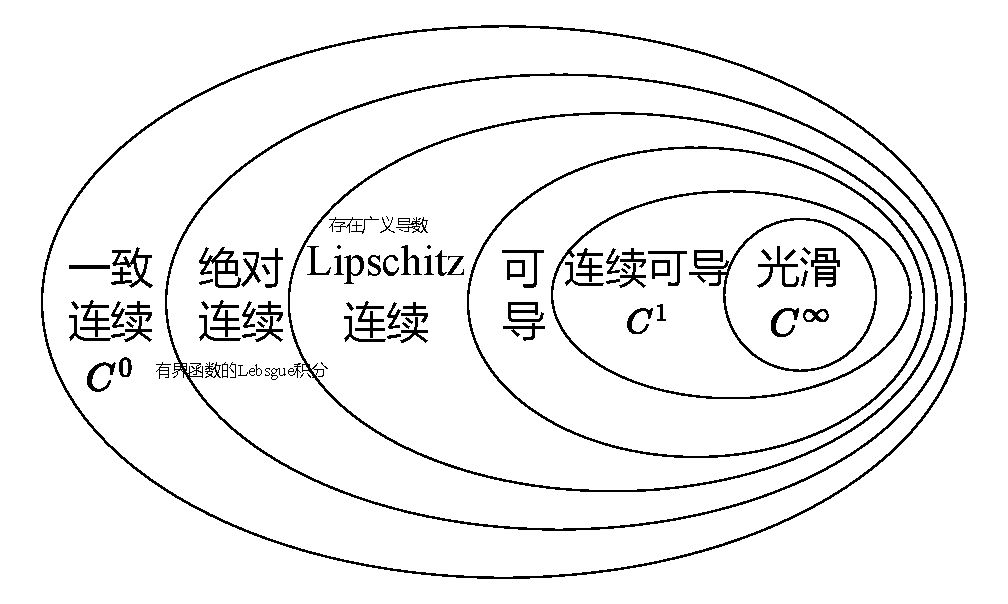
\includegraphics[width=0.6\linewidth]{asserts/连续的关系.drawio.pdf}
  \caption{控制理论中常用的连续性质的关系}
  \label{fig continuity}
\end{figure}


如下绝对值函数\(f_2(x)\)绝对连续但是在0处不可导 \[
f_2(x)=|x|, x\in [-1,1]
\]

如下根号函数绝对连续但是在0处不是局部Lipschitz连续的 \[
f_4(t)=\sqrt{|t|},t\in [0,1]
\]

\section{连续可微和光滑}

连续可微（Continuously differentiable），用泛函表示就是函数\(f\in C^1\)，意味着函数的导数是连续的，当然可微保证其本身也是连续的。

光滑函数（英语：Smooth function）在数学中特指无穷可导的函数，不存在尖点，也就是说所有的有限阶导数都存在。例如，指数函数就是光滑的，因为指数函数的导数是指数函数本身。

\begin{definition}[光滑函数]
  若一函数是连续的，则称其为\(C^{0}\)函数；
  若函数存在导函数，且其导函数连续，则称为连续可导，记为\(C^1\)函数；
  若一函数n阶可导，并且其n阶导函数连续，则为\(C^{n}\)函数（\(n\geq 1\)）。
  而光滑函数是对所有n都属于\(C^{n}\)函数，特称其为\(C^{\infty }\)函数。
\end{definition}


\section{内容概要}

从这个图可以看出在经典解中解$x(t)$是$f(x(t))$的积分，而Filippov解中$x(t)$是$f(x(t))$的Lebsgue积分。
经典解中的解是连续可导的，连续可导的意思是可导并且其导数连续，这与存在性条件$f(x(t))$连续一致。
类似地，Filippov解中解是绝对连续的，这与存在性条件$f(x(t))$可测并且局部本质有界一致。

\begin{table}[!htp]
  \centering
  \begin{tabular}{|c|c|c|c|}
    \hline
    & 解$x(t)$的连续性 & 存在性条件 & 唯一性条件 \\\hline
    经典解 & 连续可导 & 
    $f(x)$连续 & $f(x)$ Lipschitz连续\\\hline
    Filippov解 & 绝对连续 & 
    $f(x)$ 可测并且局部本质有界 & $f(x)$ Lipschitz连续 \\\hline
  \end{tabular}
  \caption{微分方程$\dot{x}=f(x)$Filippov解}
\end{table}

Every vector field that is locally Lipschitz at $x$ satisfies the one-sided Lipschitz condition on a neighborhood of $x$, but the converse is not true.

